\documentclass[10pt]{article}
\usepackage{paper}

% Set up info
\newcommand{\me}{D.~Hellfeld}
\newcommand{\papertitle}{Title of Article}
\newcommand{\university}{University of California, Berkeley}
\newcommand{\location}{Berkeley, CA 94720}
\newcommand{\department}{Nuclear Engineering}
\newcommand{\email}{dhellfeld@berkeley.edu}

% ~~~~~~~~~~~~~~~~~~~~~~~~~~~~~~~~~~~~~~~
\begin{document}

% Front matter
\frontmatter


% ============================
% Abstract
\begin{abstract}
\noindent Abstract text goes here. Abstract text goes here. Abstract text goes here. Abstract text goes here. Abstract text goes here. Abstract text goes here. Abstract text goes here. Abstract text goes here. Abstract text goes here. Abstract text goes here. Abstract text goes here. Abstract text goes here. Abstract text goes here. Abstract text goes here. Abstract text goes here. Abstract text goes here. Abstract text goes here.
\end{abstract}


% ============================
% Section 1

\section{Section Title}

Text goes here. Here is an equation
%
\begin{equation}
0! = 1
\end{equation}


% -----------------------------------------------
% Subsection 1

\subsection{Subsection Title}

Here is a citation \cite{cite1}

\begin{figure}[H]
\hypertarget{fig1}{}
\centering
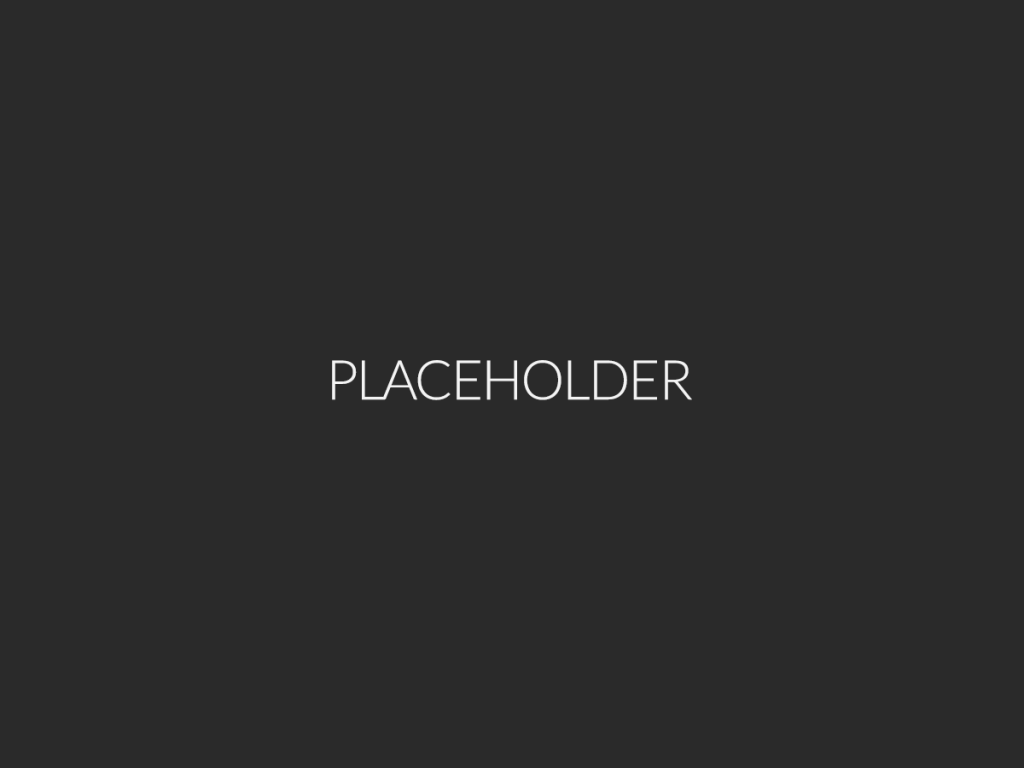
\includegraphics[width=100pt]{Figures/Placeholder.png}
\caption{Figure caption goes here.}
\end{figure}


% ============================
% References

\bibliographystyle{apsrev4-1}
\bibliography{References/references}


\end{document}
% ~~~~~~~~~~~~~~~~~~~~~~~~~~~~~~~~~~~~~~~